
\documentclass[12pt,halfline,a4paper,]{ouparticle}

% Packages I think are necessary for basic Rmarkdown functionality
\usepackage{hyperref}
\usepackage{graphicx}
\usepackage{listings}
\usepackage{xcolor}
\usepackage{fancyvrb}
\usepackage{framed}

% Link coloring
\hypersetup{breaklinks=true,
            bookmarks=true,
            pdfauthor={},
            pdftitle={STA2005S - Experimental Design Assignment}
            }


%% To allow better options for figure placement
%\usepackage{float}

% Packages that are supposedly required by OUP sty file
\usepackage{amssymb, amsmath, geometry, amsfonts, verbatim, endnotes, setspace}

% use upquote if available, for straight quotes in verbatim environments
\IfFileExists{upquote.sty}{\usepackage{upquote}}{}

% Macros for dealing with affiliations, footnotes, etc.
\makeatletter
\def\Newlabel#1#2#3{\expandafter\gdef\csname #1@#2\endcsname{#3}}

\def\Ref#1#2{\@ifundefined{#1@#2}{???}{\csname #1@#2\endcsname}}

\newcommand*\samethanks[1][\value{footnote}]{\footnotemark[#1]}

\newcommand*\ifcounter[1]{%
  \ifcsname c@#1\endcsname
    \expandafter\@firstoftwo
  \else
    \expandafter\@secondoftwo
  \fi
}

\newcommand*\thanksbycode[1]{%
  \ifcounter{FNCT@#1}
    {\samethanks[\value{FNCT@#1}]}
    {\thanks{\Ref{FN}{#1}}\newcounter{FNCT@#1}\setcounter{FNCT@#1}{\value{footnote}}}
}

% Create labels for Addresses if the are given in Elsevier format

% Create labels for Footnotes if the are given in Elsevier format

% Part for setting citation format package: natbib

% Part for setting citation format package: biblatex


% tightlist command for lists without linebreak
\providecommand{\tightlist}{%
  \setlength{\itemsep}{0pt}\setlength{\parskip}{0pt}}

% From pandoc table feature
\usepackage{longtable,booktabs,array}
\usepackage{calc} % for calculating minipage widths
% Correct order of tables after \paragraph or \subparagraph
\usepackage{etoolbox}
\makeatletter
\patchcmd\longtable{\par}{\if@noskipsec\mbox{}\fi\par}{}{}
\makeatother
% Allow footnotes in longtable head/foot
\IfFileExists{footnotehyper.sty}{\usepackage{footnotehyper}}{\usepackage{footnote}}
\makesavenoteenv{longtable}


\usepackage{float} \floatplacement{figure}{H} \usepackage{caption} \captionsetup[figure]{font=scriptsize} \pagenumbering{gobble}
\usepackage{booktabs}
\usepackage{longtable}
\usepackage{array}
\usepackage{multirow}
\usepackage{wrapfig}
\usepackage{float}
\usepackage{colortbl}
\usepackage{pdflscape}
\usepackage{tabu}
\usepackage{threeparttable}
\usepackage{threeparttablex}
\usepackage[normalem]{ulem}
\usepackage{makecell}
\usepackage{xcolor}

\begin{document}

\title{STA2005S - Experimental Design Assignment}

\author{%
%
% Code for old style authors field
%
% Add \and if both authors and author
%
%
% Code for new (elsevier) style author field
\name{Jing Yeh}
%
\email{\href{mailto:yhxjin001@myuct.ac.za}{yhxjin001@myuct.ac.za}}%
%
%
%
\and
\name{Saurav Sathnarayan}
%
\email{\href{mailto:sthsau01001@myuct.ac.za}{sthsau01001@myuct.ac.za}}%
%
%
%
%
}

\abstract{In this report, we explored the efficiency of 6 programming
languages through the approximation of \(\pi\). We found that efficiency
of various programming languages can vary widely, with C and C++ being
the most efficient programming languages. We also presented evidence for
compiled languages having better performance than interpreted languages.
Our results suggest that programmers can benefit from taking the
efficiency of various programming languages into account, rather than
simply opting for simplicity in the syntax of these languages .}

\date{2024-09-15}

\keywords{Programming Languages, Efficieny, Large-Scaled Iterative
Compuations}

\maketitle



\hfill\break
\hfill\break

\begin{center}
\includegraphics[width=100px]{pi} \end{center}
\newpage 
\tableofcontents 
\newpage

\newpage
\pagenumbering{arabic}

\section{Introduction}\label{introduction}

Computation has played a major role in human history ever since people
began living in cities. The need to calculate taxes motivated the
invention of various computing devices that aided such computations,
such as the Sumerian abacus, invented in Babylon at around 2500BC
{[}7{]}. In the 21st century, the capability of our digital computing
devices have vastly surpassed the capacity of those proto-computers, but
so has our need for computational power. Most things in our daily life
requires some form of computers: from our phones, cars, to even our
refrigerators (side note: initially, Java was invented for
refrigerators).

However, with large computation capability comes complexity in the
design of these devices: to speak plainly, they are damn difficult to
use. Computer scientists have therefore invented numerous
\emph{programming languages} that allow us to harness the power of these
devices more easily.

Nowadays, programming languages have become the primary medium for
instructing computers to perform our increasingly complex tasks.
Understanding which programming languages offer superior execution speed
is therefore crucial for developers, especially in domains requiring
real-time processing, large-scale data analysis, and other
resource-intensive computations. The goal of this experiment is to
identify such languages that deliver the fastest execution time.

\subsection{Compiled vs Interpreted
Languages}\label{compiled-vs-interpreted-languages}

In a compiled language, the source code is translated into machine code
by a compiler before execution, which produces an executable that can be
run directly by the machine. In an interpreted language, however, the
source code is executed line-by-line by its interpreter at runtime. The
interpreter reads the code, translates it into machine code, and
executes it all at once. This machine code, often called an executable,
can be run directly by the computer's hardware. Compiled languages tend
to have better performance due to the pre-compiled nature of the code,
whereas interpreted languages are more flexible but slower due to the
runtime translation

Examples: C, C++, Rust, and Java are examples of compiled languages.
Python, JavaScript, Ruby, and R are examples of interpreted languages.
\newpage

\subsection{Distribution of Execution Times (Pilot Experiment Part
1):}\label{distribution-of-execution-times-pilot-experiment-part-1}

Since existing literature on the execution times of programming
languages when applying Leibniz's formula is limited, we conducted a
mini pilot experiment on a single machine to gauge the execution times
for the programming languages we planned on experimenting with. We
performed 500 approximations, with the same algorithm, for each
programming language and obtained the following jittered graph.

\begin{figure}[H]
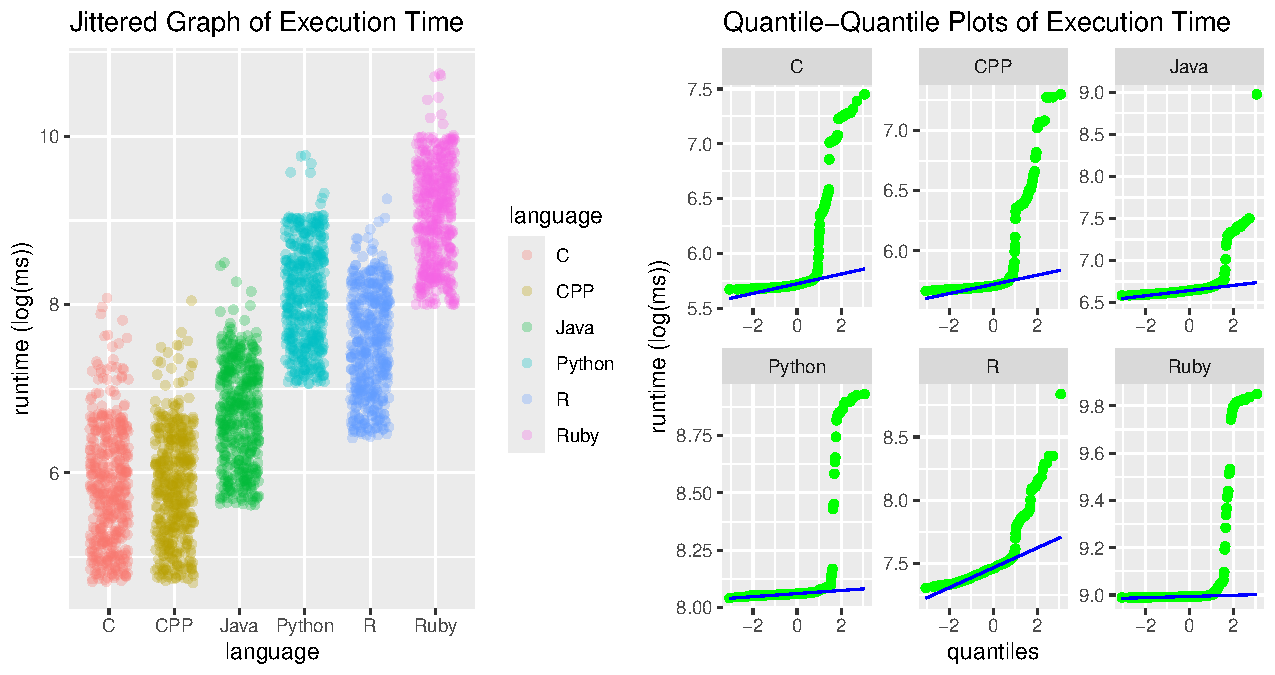
\includegraphics[width=1\linewidth]{final_files/figure-latex/figPrior-1} \caption{Runtimes of Programming Languages of Interest When Applying Leibniz's Formula up to 100 million terms}\label{fig:figPrior}
\end{figure}

We can observe that C and C++ seem to be the fastest languages on this
particular machine, though further analyses are needed. We can also see
from the Quantile-Quantile(Q-Q) plots that the execution times are
clearly not normally distributed. \newpage

\section{Methods}\label{methods}

\subsection{Setting}\label{setting}

This study was mostly conducted at the University of Cape Town,
utilising the computers available on its campus. We found that there are
only 5 different hardware setups available. Thus, to supplement the
range of our hardware setups, we also borrowed machines of 2 more
hardware setups from our friends.

\subsection{\texorpdfstring{Approximation of
\(\pi\)}{Approximation of \textbackslash pi}}\label{approximation-of-pi}

The number \(\pi\), the ubiquitous and equally mysterious irrational
number, has been fascinating the humankind since time immemorial.
Mathematicians from 4000 years ago to the present day have devised
various methods to get closer to the true value of \(\pi\). One such
method is using Leibniz's formula: \[
4 \left( 1 - \frac{1}{3} + \frac{1}{5} - \frac{1}{7} + \frac{1}{9} ±... \right) = \sum_{k=0}^{\infty}\frac{(-1)^k}{2k+1}
\] Leibniz, whom the formula is named after, proved that the series
above eventually converges to \(\pi\). That is: \[
\pi = 4 \left( 1 - \frac{1}{3} + \frac{1}{5} - \frac{1}{7} + \frac{1}{9} ±... \right) = \sum_{k=0}^{\infty}\frac{(-1)^k}{2k+1}.
\] We implemented this algorithm in 6 programming languages including 3
compiled languages: C, C++, Java, and 3 interpreted languages: Python,
R, Ruby, up to a \(100 \times 10^6\) terms. We maintained the
consistency amongst the 6 programs to the best of our ability.

\subsection{Sampling Procedure}\label{sampling-procedure}

Existing literature suggests that execution times of programming
languages are not normally distributed {[}10{]}. We confirmed this in
part I of our pilot experiment. This is an issue as it prevented us to
apply anova models. To address this, we applied the Central Limit
Theorem(CLT) to obtain a normal distribution for the average execution
times. We ran the program 15 times per sample for each programming
language, and repeated the process 30 times. Applying CLT, it is
relatively safe to assume the distribution of sample means is
approximately normal {[}8{]}. If we assume sample means to be normally
distributed, the mean of the distribution of sample means is then an
unbiased estimator for the true run time of each programming language
{[}2{]}, which we will take as a single observation. (Note: We arrived
at the number 15 through trial and error, and 30 from {[}8{]})

\subsection{Sources of Variation}\label{sources-of-variation}

\paragraph{Treatments:}\label{treatments}

We have 6 treatment factors, which are the programming languages we
applied the algorithm to. Each treatment has one level (applying the
formula up to \(100 \times 10^6\) terms). We selected this particular
level because it is the largest, practical number of terms we could
apply with our hardware setups (For some setups, it may take up to 4
hours to arrive at a single observation), and having fewer terms implies
larger relative measurement error {[}7{]}. We cannot include more levels
because in the existing literature, most studies of such kind chose to
run all languages on the same machine. However, since we would like to
avoid pseudo replication as much as possible we used one machine per
observation. The downside of this approach is that we do not have
sufficient machines to test for more than one levels.

\paragraph{Blocks:}\label{blocks}

We know that the hardware setup of a computer can significantly affect
its speed, and therefore the execution time of our algorithm. We also
know that, two computers with the same hardware setup should run at
relatively the same speed, provided that they run on the same operating
system, and no major damage has been done to either of them. This
motivated us to block for the hardware setup of computers, our
experimental units.

\subsection{Experimental Units:}\label{experimental-units}

As mentioned earlier, we would like to avoid pseudo replication as much
as possible. Therefore, we deviated from the tradition of running all
programming languages on the same machine, and test only one language
per machine. Our experimental units are therefore the individual
machines we ran each test on.

\subsection{Randomisation Procedure}\label{randomisation-procedure}

We first ordered the computers belonging to each block from 1 to 6. We
then used the random number generator from Python's \emph{random} module
to randomly shuffle, and thus producing a permutation of the list {[}C,
C++, Java, Python, Ruby, R{]}. The index of each programming language in
the permutation would then be paired to the computer with the same
assigned number.

\subsection{Planned Comparisons}\label{planned-comparisons}

We planned to conduct pairwise comparisons on all treatments. That is, a
total of \({6 \choose 2} = 15\) comparisons. We postulated that this
would help us find the most efficient language(s). It would also serve
our interest by comparing the efficiency of compiled languages (C, C++,
Java) and interpreted languages (Python, Ruby, R), as the latter are
oftentimes easier to program with. This allows us to better asses the
time-cost trade off of these programming languages.

\subsection{Pilot Experiment Part II}\label{pilot-experiment-part-ii}

We followed this direction and performed part II of our pilot study to
obtain the following execution times of programming languages on 4
hardware setups

\begin{figure}[H]
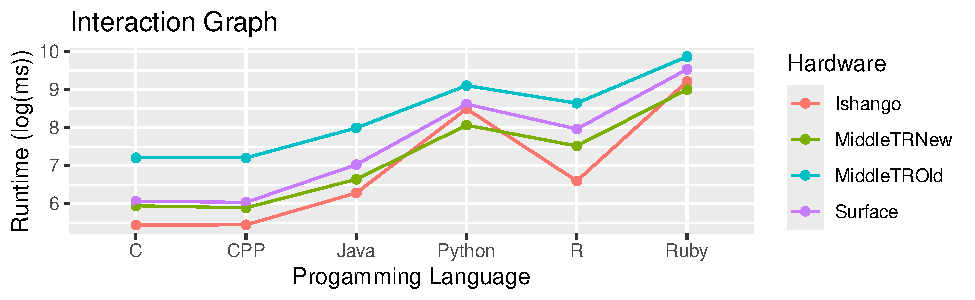
\includegraphics[width=1\linewidth]{final_files/figure-latex/figPilot-1} \caption{Interaction Graph of Programming Languages and Blocks}\label{fig:figPilot}
\end{figure}

From the data collected, we observed that the results collected from
Ishango do not follow the general trends established by the other three
setups. Firstly, the hardware setup in Ishango lab is significantly less
advance than MiddleTRNew. Yet, most programming languages tend to
perform better on the Ishango machine. Secondly, to add to the first
observation, not all programming languages perform better on the Ishango
machine.

After further investigation, we learned that programming languages
perform differently across various operating systems {[}4{]}. We
hypothesised that this is the main reason for the deviation, though
further studies are needed to confirm this (we lack access to machines
with the same hardware setup but run on different operating system).

Therefore, we added another constraint for selecting suitable machines:
the machines must all run on Windows 10, as these machines are the most
widely available. Other than than that, the results verified our
motivation for blocking various hardware setups.

\subsection{Design}\label{design}

We assume that: \[
e_{ij} \sim \mathcal{N}(0, \sigma^2)
\] We use the following anova model for our response variables:

\[
Y_{ij} = \mu + \alpha_i + \beta_j+ e_{ij}
\] \[
i = 1 ...a
\] \[
j = 1 ...b
\] With the following constraints: \[
\sum_{i=1}^a \alpha_i = \sum_{j=1}^b \beta_i =0 
\] Where: \[
\begin{aligned}
&\mu\hspace{35pt}  \text{overall mean} \\
&\alpha_i\hspace{35pt} \text{effect of }\, i^{th}\, \text{treatment}\\
&\beta_j\hspace{35pt} \text{effect of }\, j^{th}\, \text{block}\\
&e_{ij}\hspace{35pt} \text{random error of the observation}\\
\end{aligned}
\]

We also assume that each \(e_{ij}\) is independent to each other, which
allows us to assume that each \(Y_{ij}\) is also independent to each
other, and are normally distributed. If there are no blocking and
treatment effects, then: \[
Y_{ij} \sim \mathcal{N}(\mu, \sigma^2)
\] Otherwise, if there are blocking and treatment effects, then: \[
Y_{ij} \sim \mathcal{N}(\mu + \alpha_i + \beta_j, \sigma^2)
\] Below is the layout of the design:\\
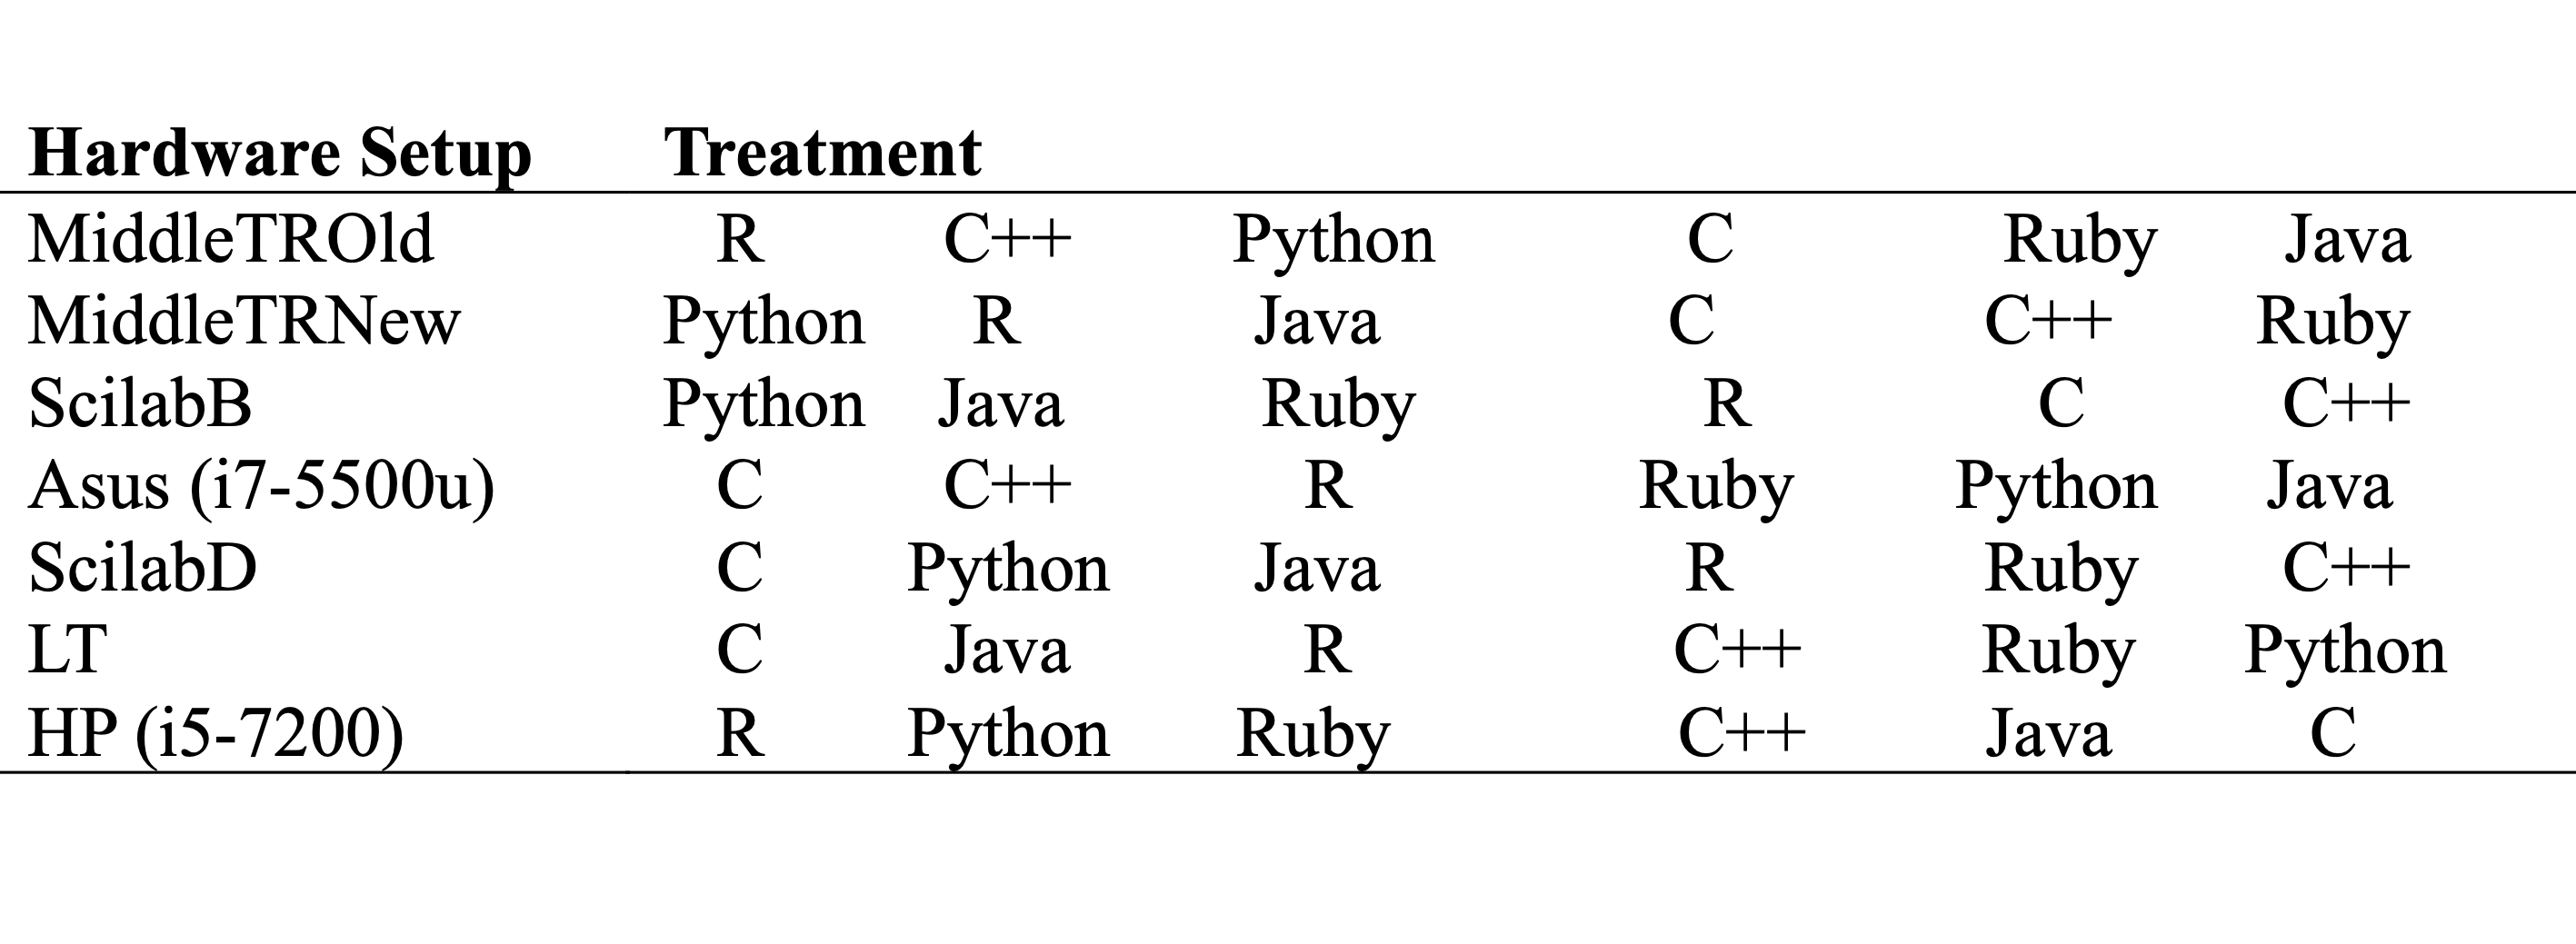
\includegraphics[width=\textwidth,height=2.08333in]{diagram.png}

\newpage

\section{Results}\label{results}

We performed the experiment described above on 7 different hardware
setups and applied all 6 treatments. Detailed tables for data and for
hardware setups can be found in the appendix. The Analysis of Variance
(ANOVA) table is shown below:

\begin{longtable}[]{@{}lrrrrr@{}}
\caption{Analysis of Variance Table}\tabularnewline
\toprule\noalign{}
& Df & Sum sq & Mean sq & F value & Pr(\textgreater F) \\
\midrule\noalign{}
\endfirsthead
\toprule\noalign{}
& Df & Sum sq & Mean sq & F value & Pr(\textgreater F) \\
\midrule\noalign{}
\endhead
\bottomrule\noalign{}
\endlastfoot
Language & 5 & 65.2112 & 13.0422 & 285.9459 & \textless{} 0.0001 \\
Hardware & 6 & 6.5717 & 1.0953 & 24.0136 & \textless{} 0.0001 \\
Residuals & 30 & 1.3683 & 0.0456 & & \\
\end{longtable}

\begin{figure}[H]

{\centering 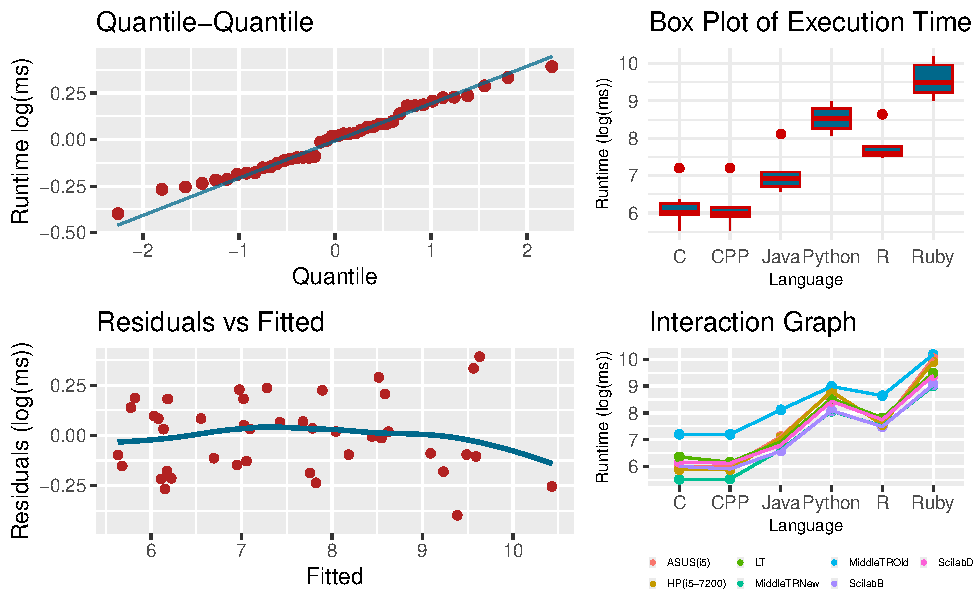
\includegraphics[width=400px]{final_files/figure-latex/figAnova-1} 

}

\caption{Diagnostic Plots}\label{fig:figAnova}
\end{figure}

\subsection{Verifying Model}\label{verifying-model}

We verified our model by observing the Fitted vs Residuals graph: the
residuals seem to be randomly spread, with no obvious patterns to be
discerned. This shows that assuming homoscedasticity (equal variance) is
not non-sensical {[}7{]}. Also, the Quantile-Quantile graph offers a
fairly good fit, providing evidence for residuals being normally
distributed.

We further verified our assumptions by performing Shapiro Wilk test to
test against the normality assumption of residuals. We obtained a fairly
large p-value of 0.7521, indicating that we have little evidence to
suggest otherwise. Further, we also got that the mean of the residuals
is extremely closed to zero ( \(< 10^{-15}\) ), indicating that it is
sensible to assume \(e_{ij} \sim \mathcal{N}(0, \sigma^2)\)

\subsection{Pairwise Comparisons}\label{pairwise-comparisons}

\begin{longtable}[]{@{}cccccc@{}}
\caption{Table of Logarithmic Mean Execution Time}\tabularnewline
\toprule\noalign{}
C & CPP & Java & Python & Ruby & R \\
\midrule\noalign{}
\endfirsthead
\toprule\noalign{}
C & CPP & Java & Python & Ruby & R \\
\midrule\noalign{}
\endhead
\bottomrule\noalign{}
\endlastfoot
2.6786 & 2.6586 & 3.0568 & 3.7041 & 4.1582 & 3.3732 \\
\end{longtable}

Given that we knew our response variables are normally distributed, we
opted for the more powerful Tukey's Method, rather than Scheffe's ,to
construct 95\% confidence intervals that compare the execution time of
every possible pair of our 6 programming languages. We use the
\emph{TukeyHSD()} function in R to achieve this. (The full table of the
output can be found in the appendix.)

We can observe that we have strong evidence to suggest that the
efficiency of various programming languages when approximating \(\pi\)
is ranked as follows.

\[
t(C) \approx t(C++) < t(Java) < t(R) < t(Python) < t(Ruby)
\] We can also see that the efficiency of programming languages can vary
significantly, with the 95\% confidence interval of the estimated
difference in execution time being between C++ and Ruby being:
\((e^{3.1058}, e^{3.4530}) = (22.32, 31.60)\). That is, C++ is between
22.32 to 31.60 times faster than Ruby at 95\% confidence level!

It would also be interesting to see, from a statistician's point of
view, which of the two most widely used languages in data analysis is
more efficient. That is, an answer to the age old question: ``Python or
R?''. We will attempt to present an answer here from the perspective of
efficiency: R is estimated to be between 2.01 to 4.03 times faster than
Python when performing our algorithm.

\subsection{Compiled vs Interpreted}\label{compiled-vs-interpreted}

We were also interested in comparing the execution times of compiled
languages and interpreted languages. The contrast, \emph{L}, can be
stated as follows: \begin{align*}
L &= \frac{1}{3} (\mu_C + \mu_{C++} + \mu_{Java}) - \frac{1}{3}(\mu_{Python} + \mu_{Ruby} + \mu_{R})\\
\intertext{We can estimate the values relevant to the contrast as follows:}
\hat{L} &= \frac{1}{3} (\bar{y}_C + \bar{y}_{C++} + \bar{y}_{Java}) - \frac{1}{3}(\bar{y}_{Python} + \bar{y}_{Ruby} + \bar{y}_{R})\\
&= -0.9198 \\
\widehat{Var(\hat{L})} &= s^{2} \sum_{i=1}^{6} \frac{{h_i}^2}{n}\\
&= 0.0456\sum_{i=1}^{6}\frac{\frac{1}{9}}{7}\\
&= 0.004343\\
SE(\hat{L}) &= \sqrt{\widehat{Var(\hat{L})}}\\
 &= \sqrt{0.004343}\\
 &= 0.0659
\end{align*} We first note that \(t_{0.025}^{30} = 2.0422\). We will
then construct a 95\% confidence interval as follows: \begin{align*}
\hat{L}&\pm SE(\hat{L})\times t_{0.025}^{30}\\
-0.9198 &\pm 0.0659 \times 2.0422\\
\intertext{Thus, the 95\% Confidence interval is as follows: }
95\%C.I. &= (-1.0544 ,-0.7852)
\end{align*}\\
The means that, at 95\% confidence level, the average execution times of
compiled languages is estimated to be between 2.19 to 2.87 times shorter
than that of the interpreted languages . We therefore have strong
evidence to suggest that compiled languages have shorter execution times
when applying Leibniz's formula up to a very large term. \newpage

\section{Discussion}\label{discussion}

The experiment aimed to analyze the execution time of different
programming languages when applying Leibniz's formula across 7 hardware
setups and 6 treatments. The ANOVA diagnostic plots (quantile-quantile
and residuals vs.~fitted) indicate a well-fitted model, with residuals
demonstrating no major deviations from our normality and
homoscedasticity assumptions, supporting the robustness of the analysis.
The ANOVA results indicate significant differences amongst the execution
times of various languages. The p value for hardware is also very low
(\textless{} 0.0001) which indicates that hardware setup does have an
effect on the execution time of different programming languages.\\
From the Tukey's HSD post-hoc tests, it is clear that C and C++ have the
fastest execution times, as reflected by their significantly lower mean
execution times compared to other languages. Java, a semi-compiled
language, performed moderately well, trailing behind C and C++ but
significantly ahead of interpreted languages like Python and Ruby. We
analysed the difference in efficiency amongst languages that serve
similar purposes, such as R and Python in data analysis, and we found,
at 95\% confidence level, that R is around 2 to 4 times faster than
Python when performing large amount of simple real number multiplication
and addition.\\
We also collected strong evidence to suggest differences in the
performance of compiled and interpreted languages. The compiled
languages (C, C++, Java) outperformed interpreted languages (R, Python,
and Ruby) by 200\% to 300\% in our results. Interpreted languages are
typically easier to program in than compiled languages and are thus
favoured by some programmers. However, our results suggest that less
difficulty in the coding stage often implies less efficiency in the
final programs produced. We thus strongly recommend programmers to take
the efficiency of various programming languages into account when
selecting one for their project.

\section{Conclusion:}\label{conclusion}

The results of this experiment confirmed that compiled languages (C and
C++) exhibit significantly faster execution times compared to both
semi-compiled (Java) and interpreted languages (R, Python, Ruby). The
performance gap between compiled and interpreted languages becomes
particularly evident with large-scale iterative computations, such as,
in our case, applying Leibniz's formula up to 100 million terms. Based
on the ANOVA and post-hoc analysis, we found, for large-scale simple
mathematical operations, that: \emph{1.}C and C++ are the most efficient
languages, followed by Java, R, Python,and then Ruby, in order.
\emph{2.}Compiled languages provide a substantial performance advantage
over interpreted languages. These findings can be useful for developers
when selecting a programming language for performance-critical
applications. \newpage

\section{Appendix}\label{appendix}

\begin{table}[ht]
\centering
\begin{tabular}{rllll}
  \hline
 & PC & CPU & RAM & OS \\ 
  \hline
1 & Ishango PC &  9th Gen Intel® Core™ i3-9100  &  8.0 GB  & Ubuntu 22.04 \\ 
  2 & MidddleTROld &  9th Gen Intel(R) Core(TM) i5-9500 CPU  &  8.0 GB  &   Windows 10 \\ 
  3 & MiddleTRNew  &  12th Gen Intel(R) Core(TM) i5-13400  &  16.0 GB  &   Windows 10 \\ 
  4 & ScilabB  &   12th Gen Intel(R) Core(TM) i5-12400  &   16.0 GB   &   Windows 10 \\ 
  5 & Surface  &   9th Gen Intel(R) Core(TM) i5-8250 CPU  &   16.0 GB   &   Windows 10 \\ 
  6 & ASUS (i7-5500u)  &   5th Gen Intel(R) Core(TM) i7-5500U CPU  &   6.0 GB   &   Windows 10 \\ 
  7 & ScilabD  &   10th Gen Intel(R) Core(TM) i5-10500  &   16.0 GB   &   Windows 10 \\ 
  8 & LT  &   9th Gen Intel(R) Core(TM) i5-9400f  &   8.0 GB   &   Windows 10 \\ 
  9 & HP (i5-7200)  &   7th Gen Intel(R) Core(TM) i5-7200  &   8.0 GB   &   Windows 10 \\ 
   \hline
\end{tabular}
\caption{Table of Pcs used and their respective specifications} 
\end{table}

\begin{table}[ht]
\centering
\begin{tabular}{rlrrrrrr}
  \hline
 & Hardware & C & CPP & Java & Python & Ruby & R \\ 
  \hline
1 & MiddleTROld & 3.13 & 3.13 & 3.53 & 3.90 & 4.42 & 3.75 \\ 
  2 & MiddleTRNew & 2.40 & 2.41 & 2.88 & 3.50 & 3.91 & 3.26 \\ 
  3 & ScilabB & 2.61 & 2.57 & 2.86 & 3.51 & 3.93 & 3.25 \\ 
  4 & ASUS(i5) & 2.61 & 2.61 & 3.09 & 3.82 & 4.35 & 3.30 \\ 
  5 & HP(i5-7200) & 2.56 & 2.56 & 3.07 & 3.82 & 4.30 & 3.29 \\ 
  6 & ScilabD & 2.68 & 2.66 & 2.96 & 3.66 & 4.08 & 3.37 \\ 
  7 & LT & 2.76 & 2.68 & 3.01 & 3.71 & 4.12 & 3.40 \\ 
   \hline
\end{tabular}
\caption{Table of data used for analysis} 
\end{table}
\begingroup\fontsize{9}{11}\selectfont

\begin{longtable}[t]{lrrrr}
\toprule
 & diff & lwr & upr & p adj\\
\midrule
CPP-C & -0.046023 & -0.393240 & 0.301194 & 0.998485\\
Java-C & 0.870722 & 0.523505 & 1.217939 & 0.000000\\
Python-C & 2.361294 & 2.014077 & 2.708512 & 0.000000\\
R-C & 1.599346 & 1.252129 & 1.946563 & 0.000000\\
Ruby-C & 3.407019 & 3.059802 & 3.754236 & 0.000000\\
\addlinespace
Java-CPP & 0.916745 & 0.569528 & 1.263962 & 0.000000\\
Python-CPP & 2.407317 & 2.060100 & 2.754534 & 0.000000\\
R-CPP & 1.645369 & 1.298152 & 1.992586 & 0.000000\\
Ruby-CPP & 3.453042 & 3.105824 & 3.800259 & 0.000000\\
Python-Java & 1.490572 & 1.143355 & 1.837789 & 0.000000\\
\addlinespace
R-Java & 0.728624 & 0.381407 & 1.075841 & 0.000007\\
Ruby-Java & 2.536297 & 2.189079 & 2.883514 & 0.000000\\
R-Python & -0.761948 & -1.109166 & -0.414731 & 0.000003\\
Ruby-Python & 1.045724 & 0.698507 & 1.392942 & 0.000000\\
Ruby-R & 1.807673 & 1.460456 & 2.154890 & 0.000000\\
\bottomrule
\multicolumn{5}{l}{\rule{0pt}{1em}Table 5: Table of Differences in Log Execution Time with Tukey's Method}\\
\end{longtable}
\endgroup{}

\newpage

\section{Reference}\label{reference}

{[}1{]} Juritz J, Little F, Erni B. Design of Experiment: Course Notes
for STA2005S. University of Cape Town; 2023.\\
\strut \\
{[}2{]} Mavuso M, Robbertze Y. Order Out of Chaos I and II: STA2004F
Notes. University of Cape Town; 2019.\\
\strut \\
{[}3{]} Dean AM, Voss D. Design and Analysis of Experiments. Springer
Science \& Business Media; 2006.\\
\strut \\
{[}4{]} Braun J. Is Linux Faster Than Windows? Speed Comparison \&
Analysis {[}Internet{]}. Linux JournalDigital. 2022. Available from:
https://www.linuxjournaldigital.com/is-linux-faster-than-windows/.\\
\strut \\
{[}5{]} Greenwood MC. Intermediate Statistics with R. 2021.\\
\strut \\
{[}6{]} Fourment M, Gillings MR. A comparison of common programming
languages used in bioinformatics. BMC Bioinformatics. 2008;9.\\
\strut \\
{[}7{]} Rhodes B. Computing is Born: The Sumerian Abacus {[}Internet{]}.
\#TechIsATool. 2020. Available from:
https://medium.com/tech-is-a-tool/the-dawn-of-computing-sumerian-abacus-83bdefb697ba.\\
\strut \\
{[}8{]} Underhill LG, Bradfield D. Introstat. University of Cape Town;
2007.\\
\strut \\
{[}9{]} Residuals vs.~Fits Plot \textbar{} STAT 501 {[}Internet{]}.
PennState: Statistics Online Courses. University of Pennsylvania;
Available from: https://online.stat.psu.edu/stat501/lesson/4/4.2.\\
\strut \\
{[}10{]} Chapter 16 - Anova {[}Internet{]}. University of South
Carolina; 2018 {[}cited 2024 Sep 14{]}. Available from:
https://www.biostat.jhsph.edu/\textasciitilde iruczins/teaching/jf/ch16.pdf.\\
\strut \\
{[}11{]} Matheus, Adriano Kamimura Suzuki. Determining the Probability
Distribution of Execution Times. 2021 IEEE Symposium on Computers and
Communications (ISCC). 2021;






\end{document}
